\documentclass[11pt,a4paper]{article}
\usepackage[margin=24mm]{geometry}
\usepackage[T1]{fontenc}
\usepackage{lmodern,amsmath,amssymb,booktabs,longtable,array,hyperref,tikz}
\usetikzlibrary{arrows.meta,positioning,shapes.gates.logic.US,calc}
\hypersetup{hidelinks,pdfauthor={Quartz-4b7e},pdftitle={Student reference report}}
\setlength{\parindent}{0pt}\setlength{\parskip}{6pt}
\newcommand{\sa}[2]{#1/\mathrm{#2}}
\title{VLSI Testing: Homework 3\\Student reference report}
\author{Quartz-4b7e}\date{}
\begin{document}\maketitle
\textbf{Status.} This is an editable English reconstruction of the anonymized student report. It preserves the student's methods and reported conclusions. Independent verification notes appear at the end and distinguish confirmed results from errors. The original statement and anonymized report are included alongside this document.
\section{Signature analysis}
\subsection{Submitted circuit and LFSR}
The report labels the six product terms of the circuit $n_1$ through $n_6$, the upper OR result $n_7$, and the lower OR result $n_8$. Line $a$ is the lower OR result before the final output OR gate. In the source, a fault control replaces $a$ with zero to emulate $a/0$.

The retained source implements the following equations, with $x_1$ corresponding to Verilog \texttt{x[0]}:
\begin{align*}
n_1&=x_1\bar x_2\bar x_3\bar x_4,&n_2&=\bar x_1\bar x_2x_3\bar x_4,\\
n_3&=x_1x_2\bar x_3x_4,&n_4&=\bar x_1x_2\bar x_3\bar x_4,\\
n_5&=\bar x_1x_2x_3x_4,&n_6&=x_1x_2\bar x_3x_4,\\
n_7&=n_1+n_2,&n_8&=n_3+n_4+n_5+n_6,\\
F_{\rm good}&=n_7+n_8,&F_{a/0}&=n_7.
\end{align*}
These are a transcription of the student RTL, not a claim that the RTL matches the statement. In particular $n_3$ and $n_6$ are identical in this source.

The modular LFSR uses characteristic polynomial $1+X+X^4$. Its four flip-flops are cleared to zero by reset. With current input $F$ and state $(D_0,D_1,D_2,D_3)$, the actual next-state equations are
\[D'_0=F\oplus D_3,\quad D'_1=D_0\oplus D_3,\quad D'_2=D_1,\quad D'_3=D_2.\]
\begin{center}
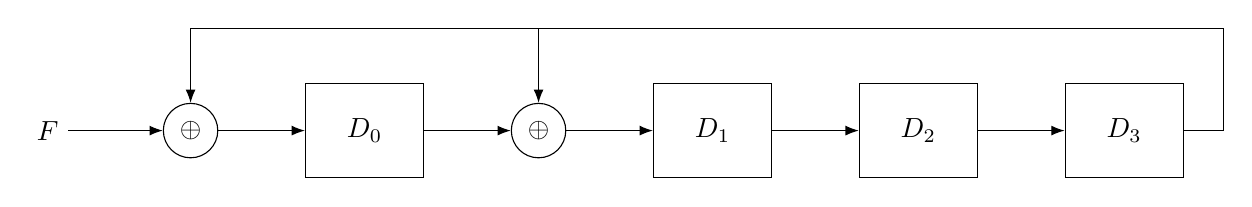
\begin{tikzpicture}[>=Latex,node distance=11mm,ff/.style={draw,minimum width=15mm,minimum height=12mm}]
\node[draw,circle] (x0) {$\oplus$};
\node[ff,right=of x0] (d0) {$D_0$};
\node[draw,circle,right=of d0] (x1) {$\oplus$};
\node[ff,right=of x1] (d1) {$D_1$};
\node[ff,right=of d1] (d2) {$D_2$};
\node[ff,right=of d2] (d3) {$D_3$};
\draw[<-](x0.west)--++(-12mm,0)node[left]{$F$};
\draw[->](x0)--(d0);\draw[->](d0)--(x1);\draw[->](x1)--(d1);
\draw[->](d1)--(d2);\draw[->](d2)--(d3);
\draw[->](d3.east)--++(5mm,0)--++(0,13mm)-|(x0.north);
\draw[->]($(d3.east)+(5mm,13mm)$)-|(x1.north);
\end{tikzpicture}\end{center}
The top-level module connects the combinational circuit to the serial signature analyzer. Two copies, one fault free and one with $a/0$, are driven by the same testbench. The counter indexes the prescribed fifteen input patterns; a sixteenth all-zero pattern is also initialized in the testbench. The signature after fifteen sampled inputs must be read before including that extra pattern.

\subsection{Report's observations}
The report gives the following chronological output sequences for the fifteen input patterns:
\begin{center}\begin{tabular}{lll}\toprule
Case&Output stream&Signature stated in report\\\midrule
Fault free&\texttt{000010001000111}&\texttt{0011}\\
$a/0$&\texttt{000000000000101}&\texttt{0010}\\\bottomrule
\end{tabular}\end{center}
The original prose then lists the faulty signature bits as 0011, creating an internal contradiction. The report concludes that differing signatures distinguish the good and faulty circuits. The independent recurrence check below resolves the actual RTL signature without silently replacing the student's text.

\section{Syndrome compaction}
The second question uses
\[e=ab,\quad f=\overline{cd},\quad z=\overline{e+f}.\]
The eight input sequences are
\[a=11110000,\quad b=11001100,\quad c=10101010,\quad d=10101110.\]
The report implements a C++ simulator. It first records the fault-free response and its parity and one's count, then injects both stuck-at values on each line $a,b,c,d,e,f,z$. Each faulty signature is compared with the good one. The following table reconstructs all output records shown in the report and produced by the submitted program.
\begin{center}
\begin{tabular}{lccc}\toprule
Fault&Output stream&Parity (one's count mod 2)&One's count\\\midrule
None&00101010&1&3\\
$a/0$&10101010&0&4\\
$a/1$&00100010&0&2\\
$b/0$&10101010&0&4\\
$b/1$&00001010&0&2\\
$c/0$&00000000&0&0\\
$c/1$&00101110&0&4\\
$d/0$&00000000&0&0\\
$d/1$&00101010&1&3\\
$e/0$&10101010&0&4\\
$e/1$&00000000&0&0\\
$f/0$&00111111&0&6\\
$f/1$&00000000&0&0\\
$z/0$&00000000&0&0\\
$z/1$&11111111&0&8\\\bottomrule
\end{tabular}\end{center}
Both compactors miss only $d/1$ in this fourteen-fault model. Its full output stream is already identical to the good response, so neither parity nor one's count can reveal it. Every other fault produces even parity and a one's count different from three. The report's stated conclusion for question 2 is therefore consistent with these results.

\section{Independent verification notes}
Direct evaluation of the fifteen original statement vectors gives the good-output stream stated in its table as \texttt{110000011010110}. The submitted RTL instead gives \texttt{000010001000111}. For example, the first vector 0001 has stated output one but every product term in the submitted source is zero. Thus the implementation is a reference with a real circuit mismatch, not a validated solution to question 1.

Applying the exact retained LFSR recurrence from zero to the student's good output gives 0011. Applying it to the student's faulty output gives 1010. This differs from both faulty-signature descriptions in the original report. Bit order here is explicitly $(D_0,D_1,D_2,D_3)$ and streams are in chronological test order.

The C++ program builds under C++17 and runs over its intended fault indices zero through fourteen. Compiler warnings identify an unused array and a potentially uninitialized output outside that domain. The program also allocates signature arrays without freeing them. Those issues are retained with the original source; the finite intended-domain output is still independently checkable.

\section{Retained files}
The source directory contains \texttt{circuit.v}, \texttt{LFSR.v}, \texttt{HW3\_1.v}, \texttt{HW3\_1\_tb.v}, and \texttt{HW3\_2.cpp}. The testbench uses FSDB dumping tasks. The extensionless compiled C++ executable is excluded because it is a build artifact. No simulator project or cache is required to rebuild these sources.
\end{document}
